\documentclass{beamer}
%Для защит онлайн лучше использовать разрешение 16x9
%\documentclass[aspectratio=169]{beamer}

%%% Обязательные пакеты
%% Beamer
\usepackage{beamerthemesplit}
\usetheme{SPbGU}
\beamertemplatenavigationsymbolsempty
\usepackage{appendixnumberbeamer}

%% Локализация
\usepackage{fontspec}
\setmainfont{CMU Serif}
\setsansfont{CMU Sans Serif}
\setmonofont{CMU Typewriter Text}
%\setmonofont{Fira Code}[Contextuals=Alternate,Scale=0.9]
%\setmonofont{Inconsolata}
% \newfontfamily\cyrillicfont{CMU Serif}

\usepackage{polyglossia}
\setdefaultlanguage{russian}
\setotherlanguage{english}

%% Графика
\usepackage{wrapfig} % Позволяет вставлять графику, обтекаемую текстом
\usepackage{pdfpages} % Позволяет вставлять многостраничные pdf документы в текст

%% Математика
\usepackage{amsmath, amsfonts, amssymb, amsthm, mathtools} % "Адекватная" работа с математикой в LaTeX

% Математические окружения с русским названием
\newtheorem{rutheorem}{Теорема}
\newtheorem{ruproof}{Доказательство}
\newtheorem{rudefinition}{Определение}
\newtheorem{rulemma}{Лемма}


%%% Дополнительные пакеты. Используются в презентации, но могут быть отключены при необходимости
\usepackage{tikz} % Мощный пакет для создание рисунков, однако может очень сильно замедлять компиляцию
\usetikzlibrary{decorations.pathreplacing,calc,shapes,positioning,tikzmark}

\usepackage{multirow} % Ячейка занимающая несколько строк в таблице

%% Пакеты для оформления алгоритмов на псевдокоде
\usepackage[noend]{algpseudocode}
\usepackage{algorithm}
\usepackage{algorithmicx}

\usepackage{fancyvrb}


% То, что в квадратных скобках, отображается внизу по центру каждого слайда. 
\title[Короткое название]{Полный официальный заголовок квалификационной работы}

% То, что в квадратных скобках, отображается в левом нижнем углу. 
\institute[СПбГУ]{}

% То, что в квадратных скобках, отображается в левом нижнем углу.
\author[Василий Пупкин]{Василий Иванович Пупкин, группа ХХ.БХХ-мм}
 
\begin{document}
{
\setbeamertemplate{footline}{}
% Лого университета или организации, отображается в шапке титульного листа
\begin{frame}
  
\includegraphics[width=1.4cm]{pictures/SPbGU_Logo.png}
\vspace{-35pt}
\hspace{-10pt}
\begin{center}
   \begin{tabular}{c}
        \scriptsize{Санкт-Петербургский государственный университет} \\
        \scriptsize{Кафедра системного программирования}
    \end{tabular}
\titlepage
\end{center}

\btVFill

{\scriptsize
  % У научного руководителя должна быть указана научная степень
   \textbf{Научный руководитель:} к.ф.-м.н. А.А. Андреев, доцент кафедры системного программирования \\
  % Консультанта может и не быть. Должна быть указана должность или ученая степень
   \textbf{Консультант:}  П.П. Петров, программист ЗАО \enquote{Компания с ну очень-очень-очень длинным названием}\\
  % Для курсовой не обязателен. Должна быть указана должность или ученая степень
   \textbf{Рецензент:} д.т.н., проф. И.И. Иванов, исполнительный директор ООО \enquote{Рога и копыта}  
 }
\begin{center}
  \vspace{5pt}
  \scriptsize{Санкт-Петербург\\
                 2023}
  \end{center}

\end{frame}
}

\begin{frame}[fragile]  
  \frametitle{Введение}
  \begin{itemize}
    \item Краткий обзор тематики работы (как вариант~--- устно, пока показывается титульный слайд)
    \item Не нужно определять общеизвестные понятия
    \item Применимость/полезность данной работы, обоснование выбора именно этой темы 
    \item Если тема похожа на темы других работ (в том числе прошлых лет), надо явно описать разницу
  \end{itemize}
\end{frame}
            
\begin{frame}  
  \frametitle{Существующие решения (инструменты, подходы, алгоритмы)}
  \begin{itemize}
    \item Перечислить инструменты/подходы, применяемые в области
    \item Указать их преимущества и недостатки (критика существующих решений/подходов)    
  \end{itemize}
    
\end{frame}

\begin{frame}  
  \frametitle{Существующие решения}
  Возможно, предметная область сложна и потребуется больше одного слайда, но затягивать введение не стоит. Постарайтесь уложиться в 1--2 слайда
  \begin{itemize}
    \item Выводы
    \begin{itemize}
      \item Подвести итог
      \item Указать недостатки существующих подходов, на борьбу с которыми 
направленна данная работа
      \item Чётко сформулировать существующую проблему, которая будет решаться в данной работе
    \end{itemize}
  \end{itemize}
\end{frame}


% Обязательный слайд: четкая формулировка цели данной работы и постановка задачи
% Описание выносимых на защиту результатов, процесса или особенностей их достижения и т.д.
\begin{frame}
  \frametitle{Постановка задачи}
  \textbf{Целью} работы является решение какой-то проблемы %озвученной выше  

  \textbf{Задачи}:
  \begin{itemize}
    \item Выбрать алгоритм, подход, метод %основываясь на проведённом анализе проблемы, области, существующих решений
    \item Разработать алгоритм, делающий то-то с тем-то
    \item Доказать корректность алгоритма
    \item Реализовать предложенный алгоритм
    \item Провести экспериментальное исследование предложенной реализации 
  \end{itemize}
\end{frame}
            
%Идеально, если есть по одному слайду на каждую поставленную задачу            

\begin{frame}
  \frametitle{Алгоритм ABC\footnote{Результаты и обоснования выбора пути достижения цели}}
  За основу решения взят алгоритм ABC
  \begin{itemize}
    \item Почему именно он, а не другие
    \item Ключевые особенности выбранного алгоритма, важные для решения поставленных задач    
  \end{itemize}
\end{frame}


\begin{frame}[fragile]
\frametitle{Новый алгоритм\footnote{Иллюстративные возможности: таблицы, картинки, код}}
% Задается ширина столбцов
\begin{tabular}{p{5cm} p{7cm}}
% Фрагмент кода
\begin{minipage}{3in}
  \begin{Verbatim}[commandchars=\\\{\}]

\textcolor{blue}{string} res = \textcolor{orange}{""};
\textcolor{blue}{for}(i = 0; i < l; i++) \{
    res = \textcolor{orange}{"()"} + res;
\}   

  \end{Verbatim}
\end{minipage}
&
Результат (SPPF):
\\
Аппроксимация: 
&
% Картинка. Изображения должны быть векторными. Исключения --- снимки экрана.
\multirow{-2}*{\!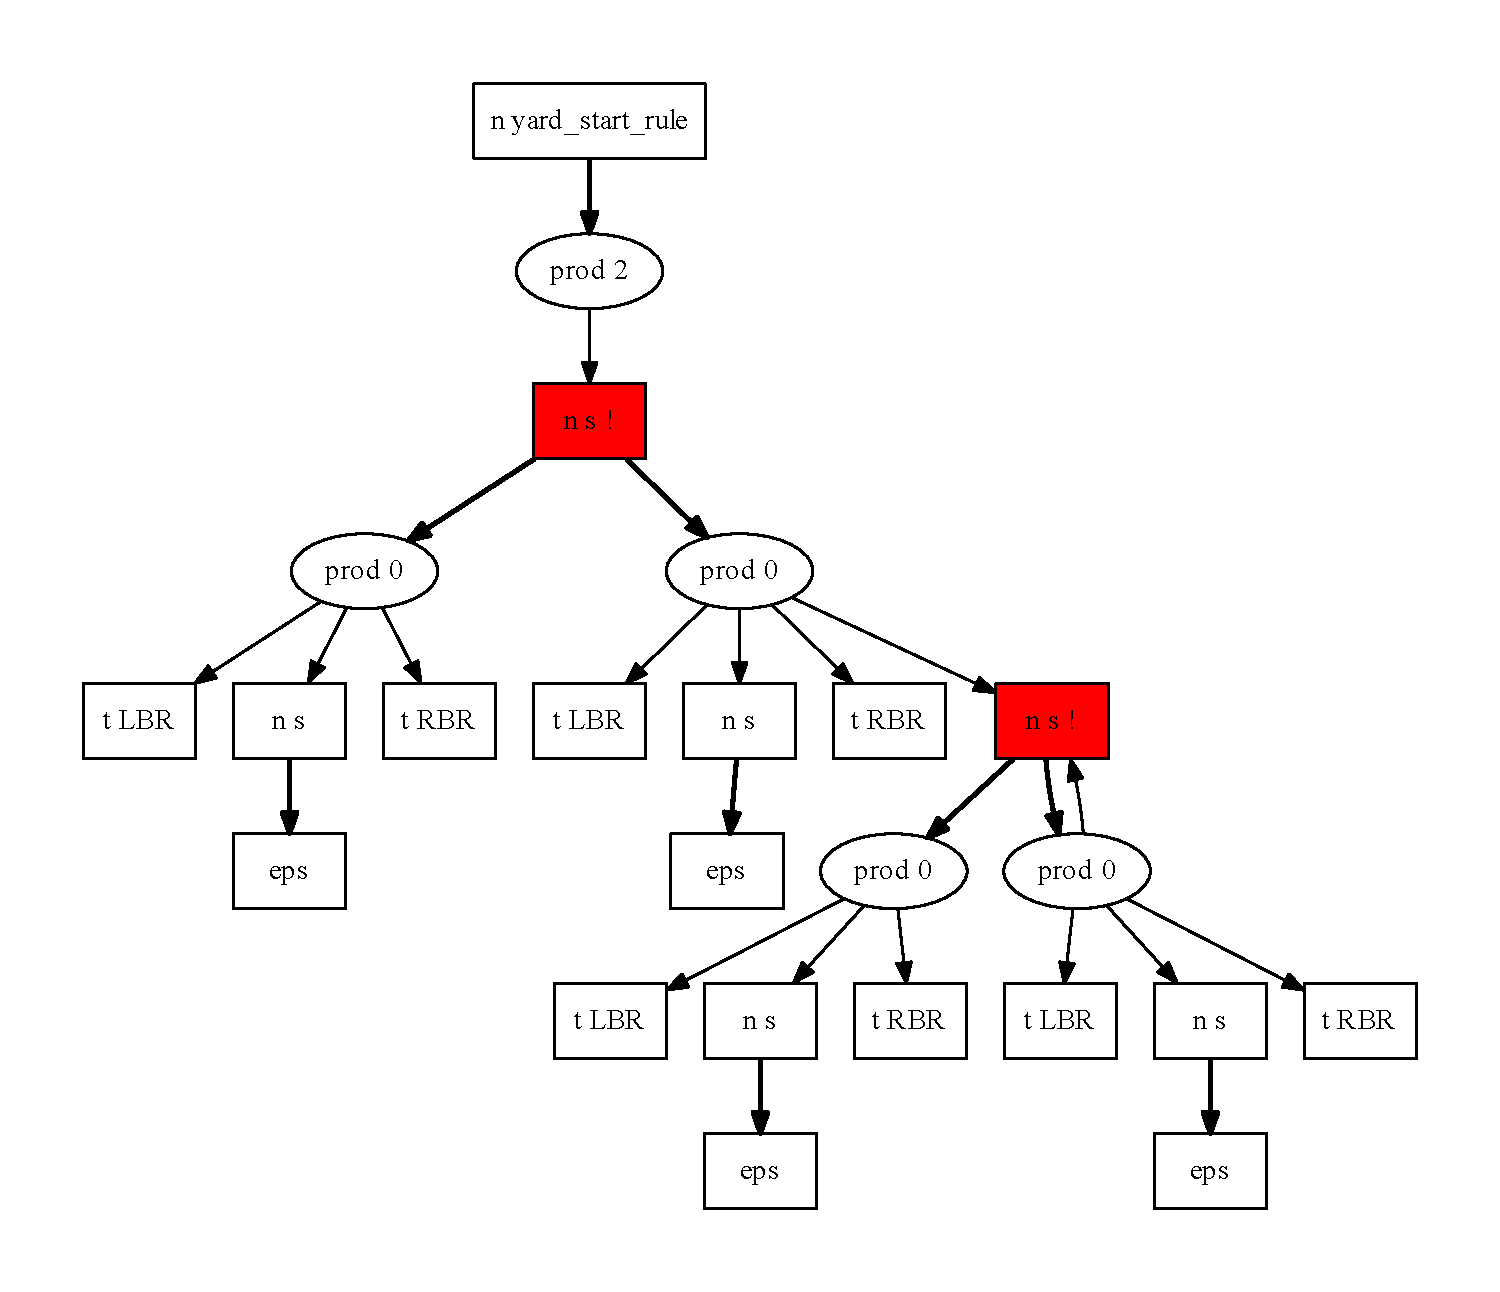
\includegraphics[width=6.8cm]{pictures/out3.pdf}}
\\
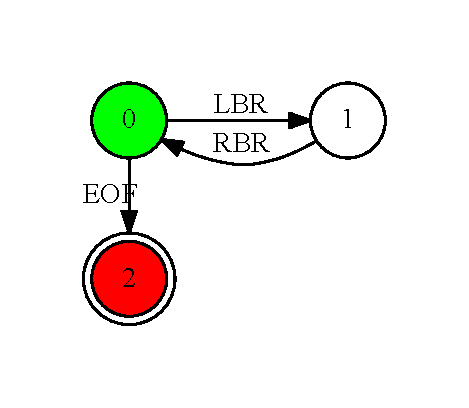
\includegraphics[width=2.5cm]{pictures/in3.pdf}
&
\\      
Грамматика: &
\\
\vspace{-20pt}
% Можно формулы писать
{\begin{align*}
  start& & &\Coloneq & &s \\
  s & & &\Coloneq & &\mbox{\texttt{LBR }} s \mbox{\texttt{ RBR }} s \\
  s & & &\Coloneq & &\epsilon
\end{align*}}
& 
\end{tabular}
\end{frame}

\begin{frame}[fragile]
  \frametitle{Доказательство корректности алгоритма}
  {\tiny Формулировки утверждений. Идеи доказательств проговариваются устно.}
  \begin{rutheorem}[Пифагора: геометрическая формулировка]
    В прямоугольном треугольнике площадь квадрата, построенного на гипотенузе, равна сумме площадей квадратов, построенных на катетах.
  \end{rutheorem}

  \begin{rutheorem}[Пифагора: алгебраическая формулировка]
    В прямоугольном треугольнике квадрат длины гипотенузы равен сумме квадратов длин катетов.    

    То есть, если обозначить длину гипотенузы треугольника через $c$, а длины катетов 
через $a$ и $b$, получим верное равенство: $a^2 + b^2 = c^2$.
  \end{rutheorem}

  \begin{rutheorem}[Обратная теорема Пифагора]
    Для всякой тройки положительных чисел $a$, $b$ и $c$, такой, что $a^2 + b^2 = c^2$, существует прямоугольный треугольник с катетами $a$ и $b$ и гипотенузой $c$.
  \end{rutheorem}  
\end{frame}

\begin{frame}[fragile]
  \frametitle{Архитектура решения}
  \begin{itemize}
    \item В реализации интересны архитектура, библиотеки, инструменты
    \item Не надо добавлять на слайд примеры кода
  \end{itemize}
  \begin{center}
  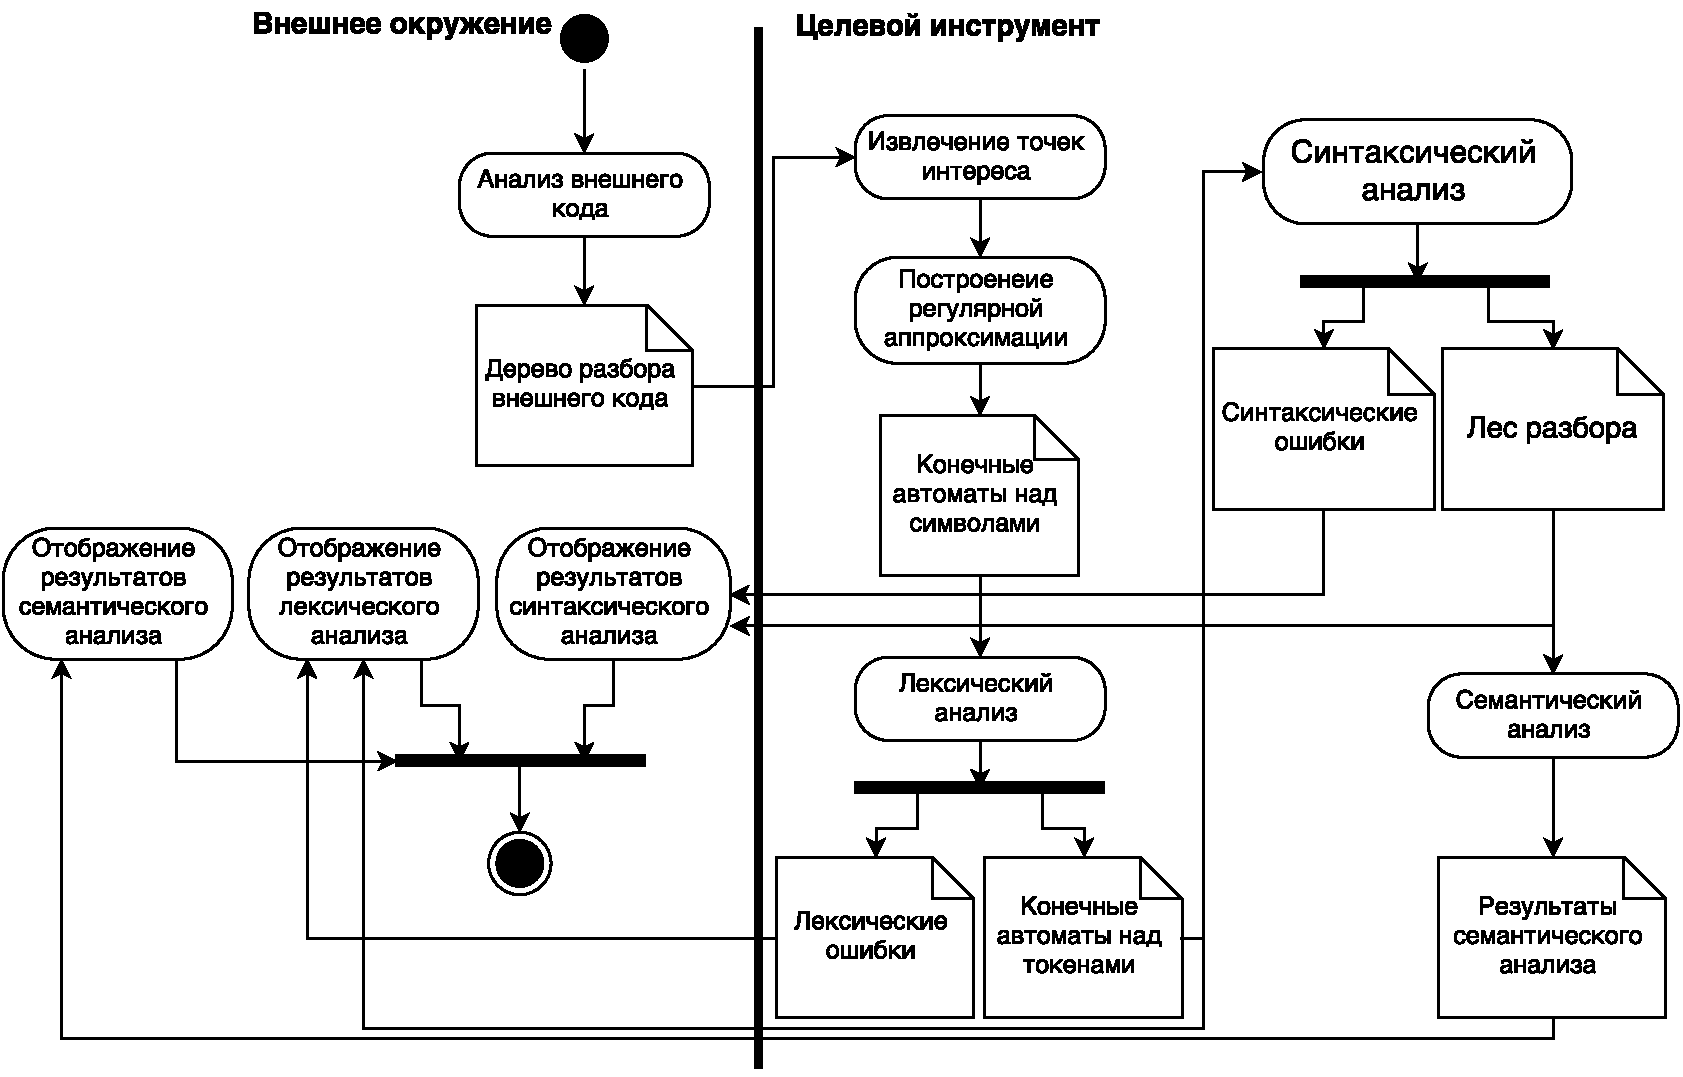
\includegraphics[width=0.8\textwidth]{pictures/Activ_SEL_Processing.pdf}
  \end{center}
\end{frame}

\begin{frame}[t]
  \frametitle{Экспериментальное исследование}
  Постановка эксперимента
  \begin{itemize}
    \item На каком наборе данных проводилось экспериментальное исследование, почему были выбраны именно эти данные    
    \item На каком оборудовании проводилось исследование    
    \item Какие решения были выбраны для сравнения и почему
  \end{itemize}  
\end{frame}

\begin{frame}[t]
  \frametitle{Результаты экспериментального исследования}
  \begin{itemize}  
    \item Какие результаты показало экспериментальное исследование
    \item Желательно привести графики, иллюстрирующие полученные результаты
    \begin{itemize}
      \item У иллюстраций должны быть подписи, у графиков~--- легенда, подписи к осям, например:
    \end{itemize}
  \end{itemize}
  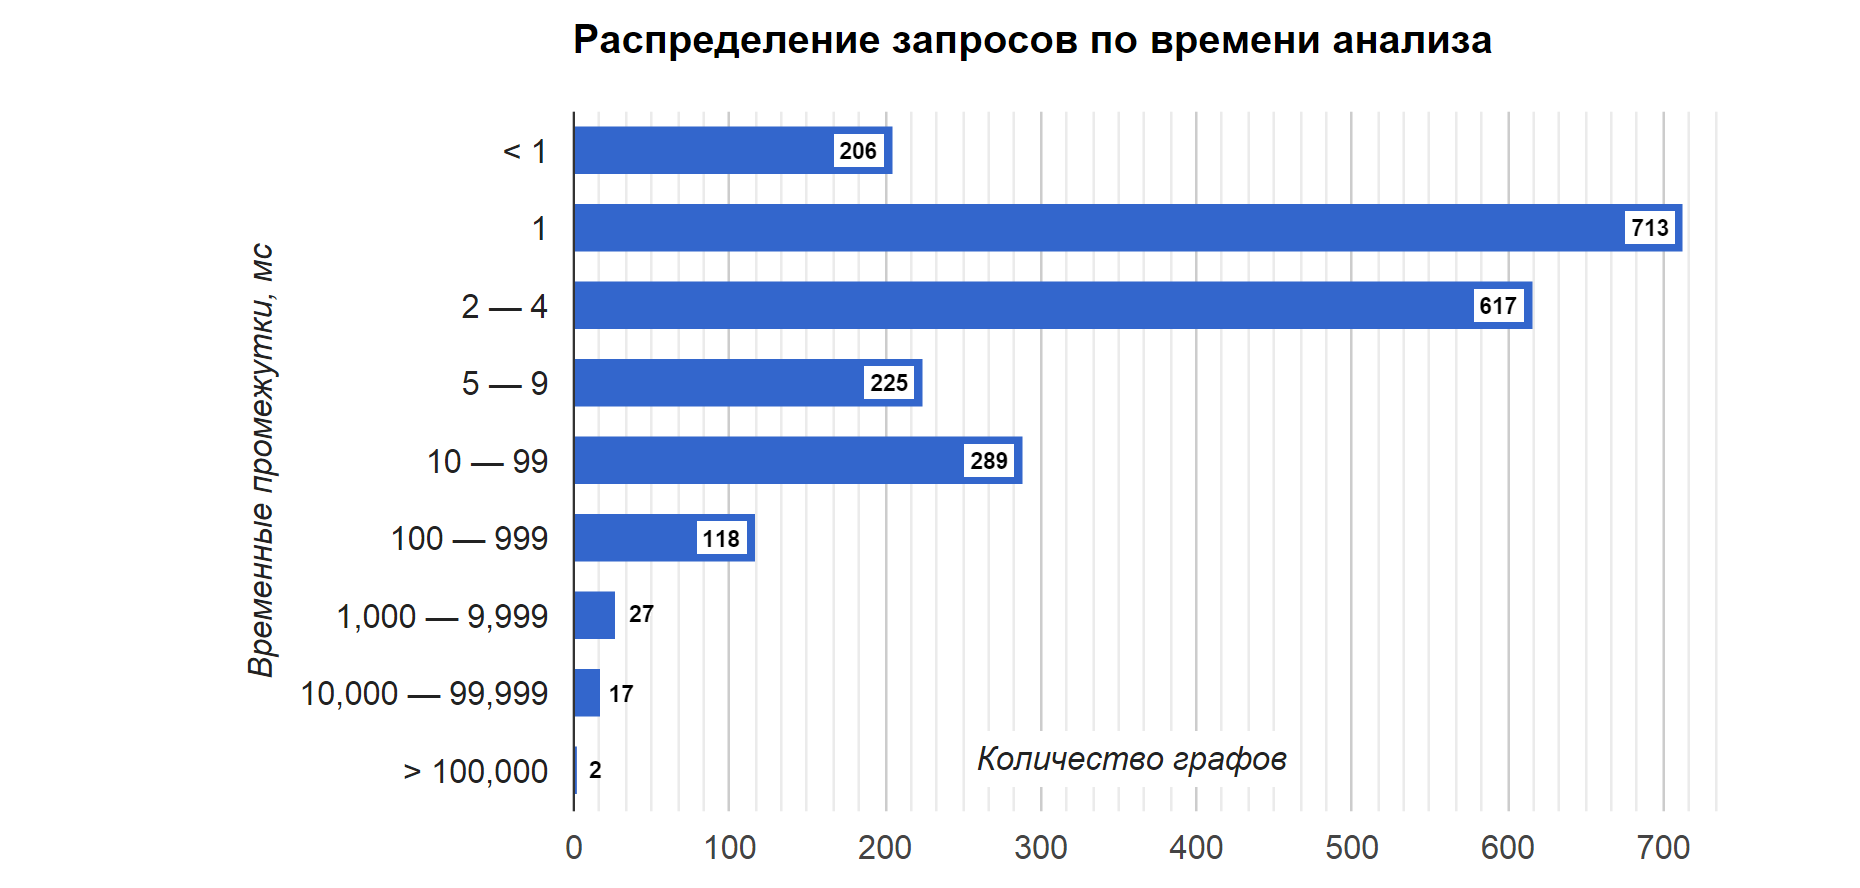
\includegraphics[width=10cm]{pictures/dist.png}
\end{frame}


\begin{frame}
  \frametitle{Результаты}
  \begin{itemize}
    \item Практически то же, что и на слайде с постановкой задачи, но в совершенной форме~--- что делал лично автор
    \item Четкое отделение результатов своей работы (особенно для коллективных работ)
      \item Формулировать глаголами совершенного вида в прошедшем времени (\enquote{сделано}, \enquote{получено})
    \item Обсуждение (ограничения, валидность, альтернативы)
    \item Не нужно слайдов типа \enquote{Все}, \enquote{Вопросы?}, \enquote{Спасибо за внимание}
  \end{itemize}

  \begin{itemize}
    \item Если результаты были представлены на конференции и опубликованы, это желательно указать 
  \end{itemize}
\end{frame}

%\addtocounter{framenumber}{1}
\appendix

\begin{frame}
  \frametitle{Дополнительный слайд}
  Например, с огромной страшной формулой всего, которая нужна для пояснения деталей при ответе на частый вопрос
  
\begin{align*}
  \MoveEqLeft \lim_{\bigtriangleup t \to 0^+}\int_{\bigtriangleup t}^{T} \! \int_{\Omega} \! D(t_1,x) \frac{\varphi(t_1-\bigtriangleup t,x)-\varphi(t_1,x)}{(-\bigtriangleup t)} \, \mathrm{d}x \, \mathrm{d}t_1 \\
  &= \lim_{\bigtriangleup t \to 0^+} \int_{0}^{T} \! \int_{\Omega} \! D(t_1,x) \frac{\varphi(t_1-\bigtriangleup t,x)-\varphi(t_1,x)}{(-\bigtriangleup t)} \chi_{(\bigtriangleup t,T)}(t_1) \, \mathrm{d}x \, \mathrm{d}t_1 \\
  &=\int_{0}^{T} \! \int_{\Omega} \! D(t_1,x) \frac{\partial \varphi}{\partial t_1} (t_1,x) \, \mathrm{d}x \, \mathrm{d}t_1 .
\end{align*}
\end{frame}

\begin{frame}
  \frametitle{Второй дополнительный слайд}
\begin{itemize}
  \item Много дополнительных слайдов не надо: 1--2 вполне достаточно в большинстве случаев
  \item Кроме формул здесь могут быть схемы, рисунки, таблицы и другие вспомогательные материалы
\end{itemize}

\end{frame}

\begin{frame}
  \frametitle{Анимация}
  Чаще всего анимированные слайды не требуются, но если очень надо, возможность добавить анимацию в PDF есть.
  Используйте анимацию на слайдах с умом и только в случае необходимости (см. комментарий в исходном тексте)
  % !!! ВНИМАНИЕ !!!
  % Для воспроизведения анимированных иллюстраций необходимо использовать просмотрщик PDF, поддерживающий исполнение скриптов, например
  % - Adobe Acrobat Reader
  % - Okular
  %
  % Проблема в том, что многие популярные просмотрщики это делать не умеют, например
  % - Evince
  % - Web-браузеры
  %
  % Часто показывать презентацию вы будете не со своего компьютера, на котором может не быть подходлящего просмотрщика.
  % Поэтому пользуйтесь анимацией на свой страх и риск!!!
  %
  % Полезные материалы
  % - https://tug.ctan.org/macros/latex/contrib/animate/animate.pdf — документация к пакету animate
  % - https://texblog.org/2018/03/05/the-animate-package/ — коротенький гайд для минимального примера

  \setlength{\fboxsep}{0pt}
  \setlength{\fboxrule}{0.5pt}
  \begin{figure}[h]
    \begin{minipage}{0.45\textwidth}
        \centering
        \fbox{\animategraphics[autoplay, loop, scale=0.3]{7}{pictures/sensors/sensors-}{1}{26}}
    \end{minipage}
    \begin{minipage}{0.45\textwidth}
        \centering
        \fbox{\animategraphics[autoplay, loop, scale=0.3]{7}{pictures/encoders/encoders-}{1}{24}}
    \end{minipage}
    \caption{Сенсоры и энкодеры}
  \end{figure}
\end{frame}

\end{document}
